\documentclass[]{article}
\usepackage{graphicx}
\usepackage{caption}
\usepackage{subcaption}

%opening
\title{Computer Vision: Project 1}
\author{Ibraheem Muhammad Moosa}

\begin{document}

\maketitle

\section{Custom Mirrors}

In the following figures we show our intermediate results on the Custom Mirrors image. At first many keypoints are detected by the scale space extremum algorithm(Figure~\ref{custommirrorsleftstep1} and Figure~\ref{custommirrorsrightstep1}). Then we filter out the low contrast and edge pixels(Figure~\ref{custommirrorsleftstep2} and Figure~\ref{custommirrorsrightstep2}). Then we calculate the orientations of each of the keypoints(Figure~\ref{custommirrorsleftstep3} and Figure~\ref{custommirrorsrightstep3}). Finally, we show the matched keypoints in Figure~\ref{custommirrorsleftstep4} and Figure~\ref{custommirrorsrightstep4}.
%\subsection{Initial Keypoints}
\begin{figure}[htb]
	\centering
	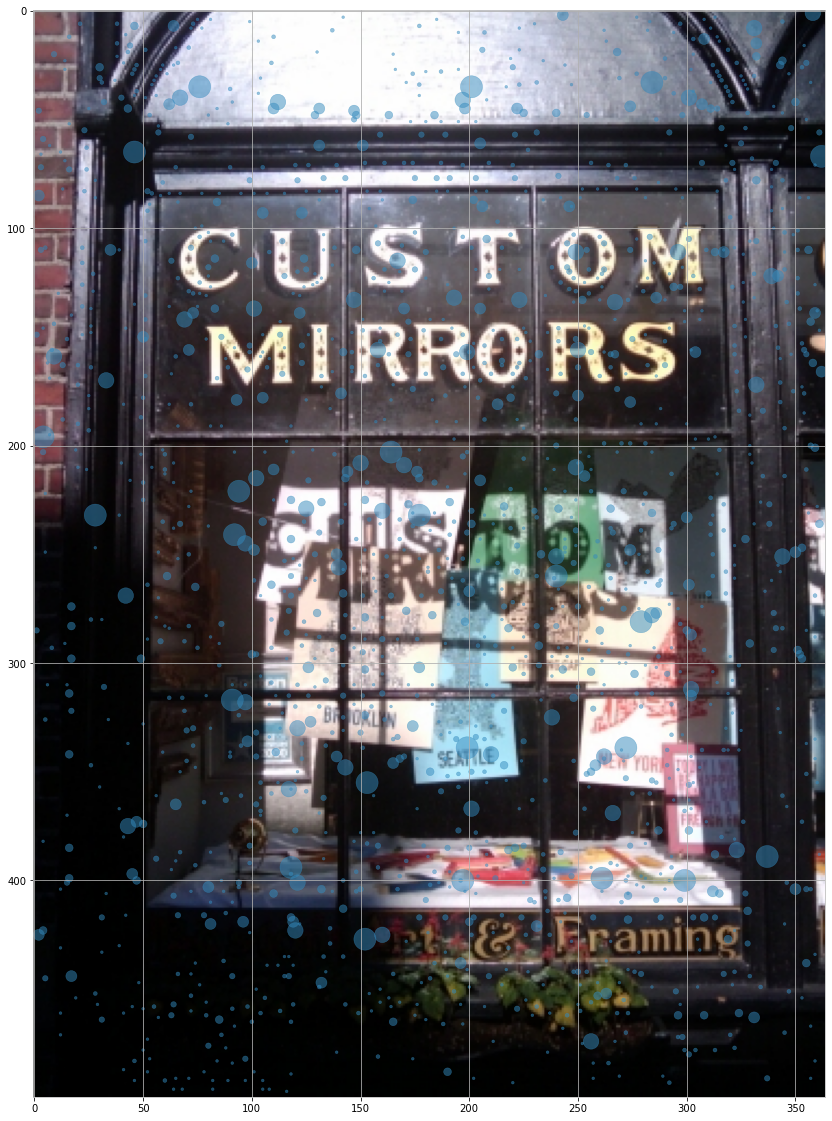
\includegraphics[width=\linewidth]{CustomMirrorsLeftStep1}
	\caption{Left image initial keypoints}
	\label{custommirrorsleftstep1}
\end{figure}
\begin{figure}[htb]
	\centering
	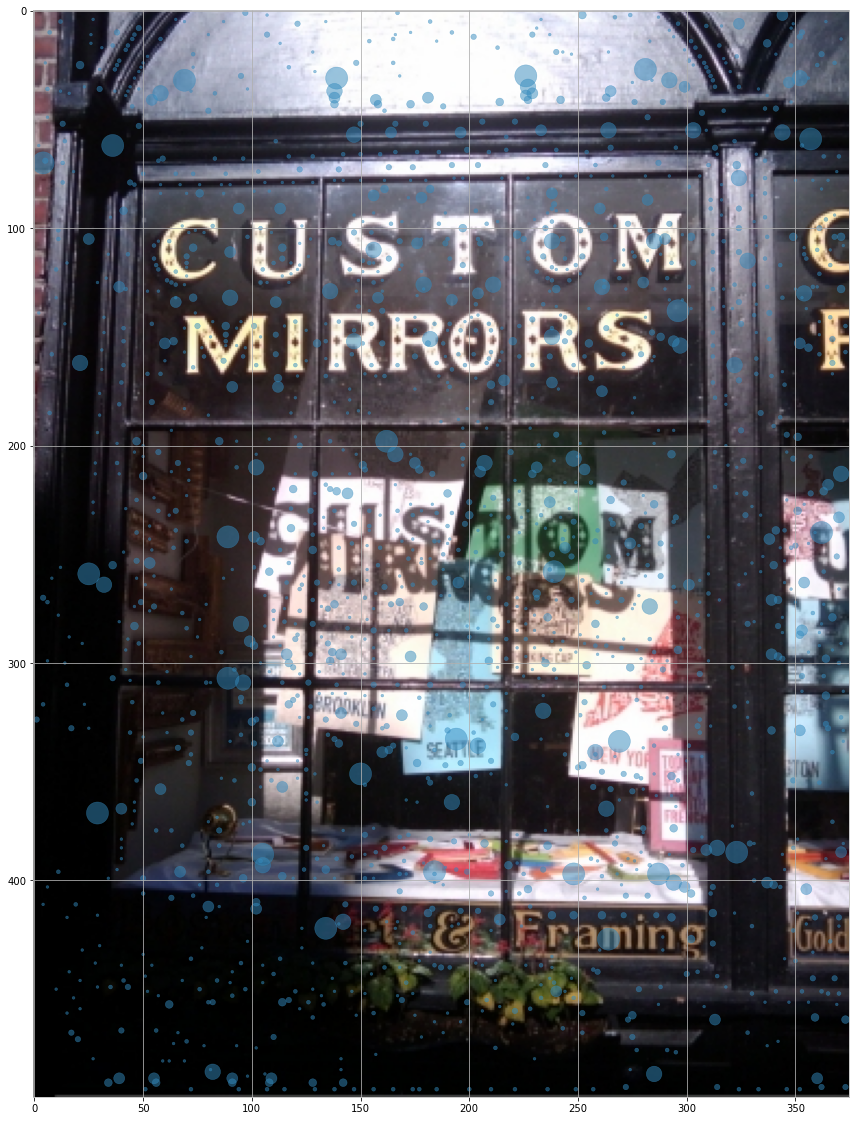
\includegraphics[width=\linewidth]{CustomMirrorsRightStep1}
	\caption{Right image initial keypoints}
	\label{custommirrorsrightstep1}
\end{figure}

%\newpage
%\subsection{Keypoints after localization}
\begin{figure}[htb]
	\centering
	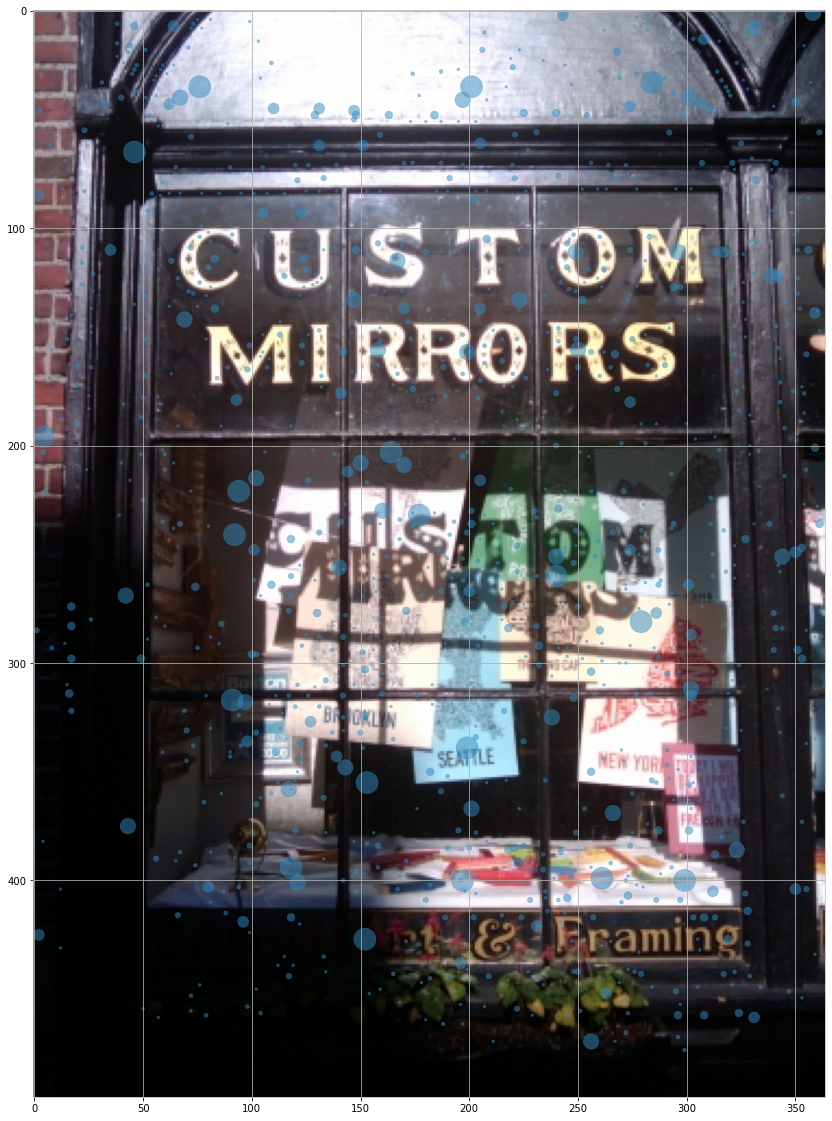
\includegraphics[width=\linewidth]{CustomMirrorsLeftStep2}
	\caption{Left image keypoints after localization}
	\label{custommirrorsleftstep2}
\end{figure}
\begin{figure}[htb]
	\centering
	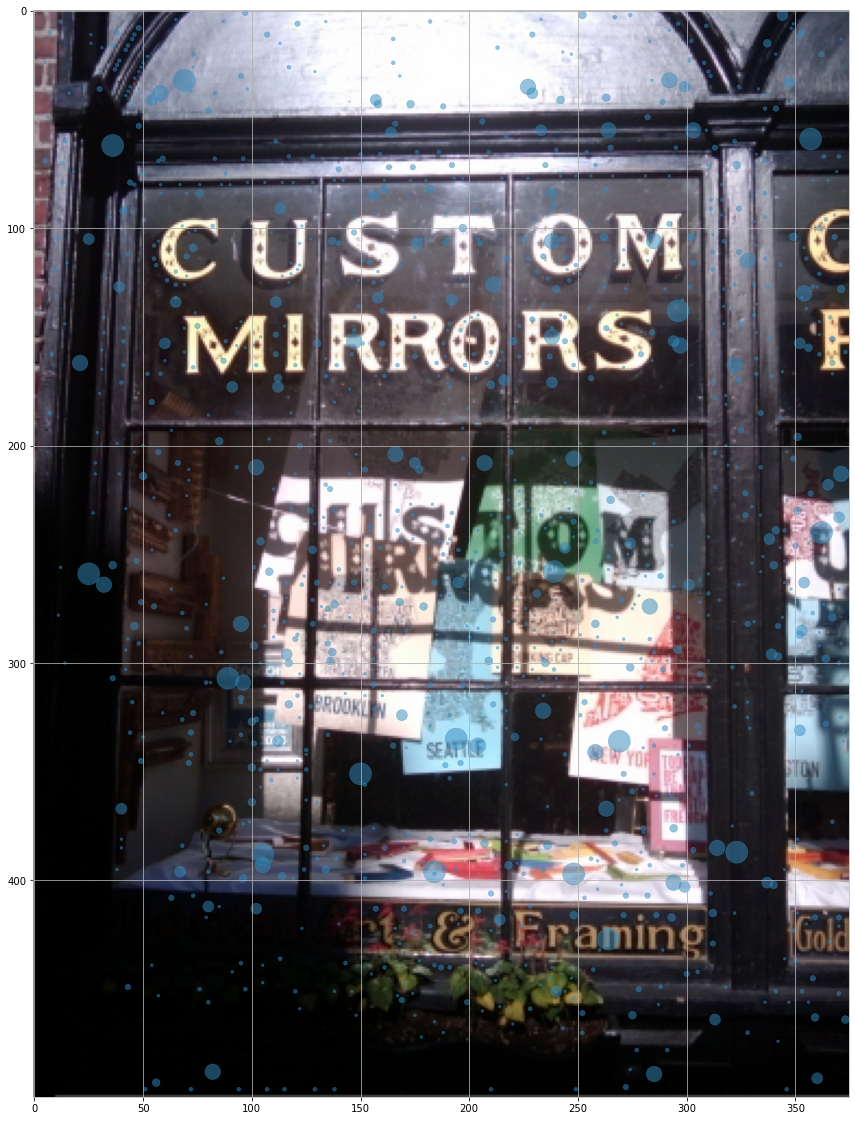
\includegraphics[width=\linewidth]{CustomMirrorsRightStep2}
	\caption{Right image keypoints after localization}
	\label{custommirrorsrightstep2}
\end{figure}

%\newpage
%\subsection{Keypoints with orientation assignment}
\begin{figure}[htb]
	\centering
	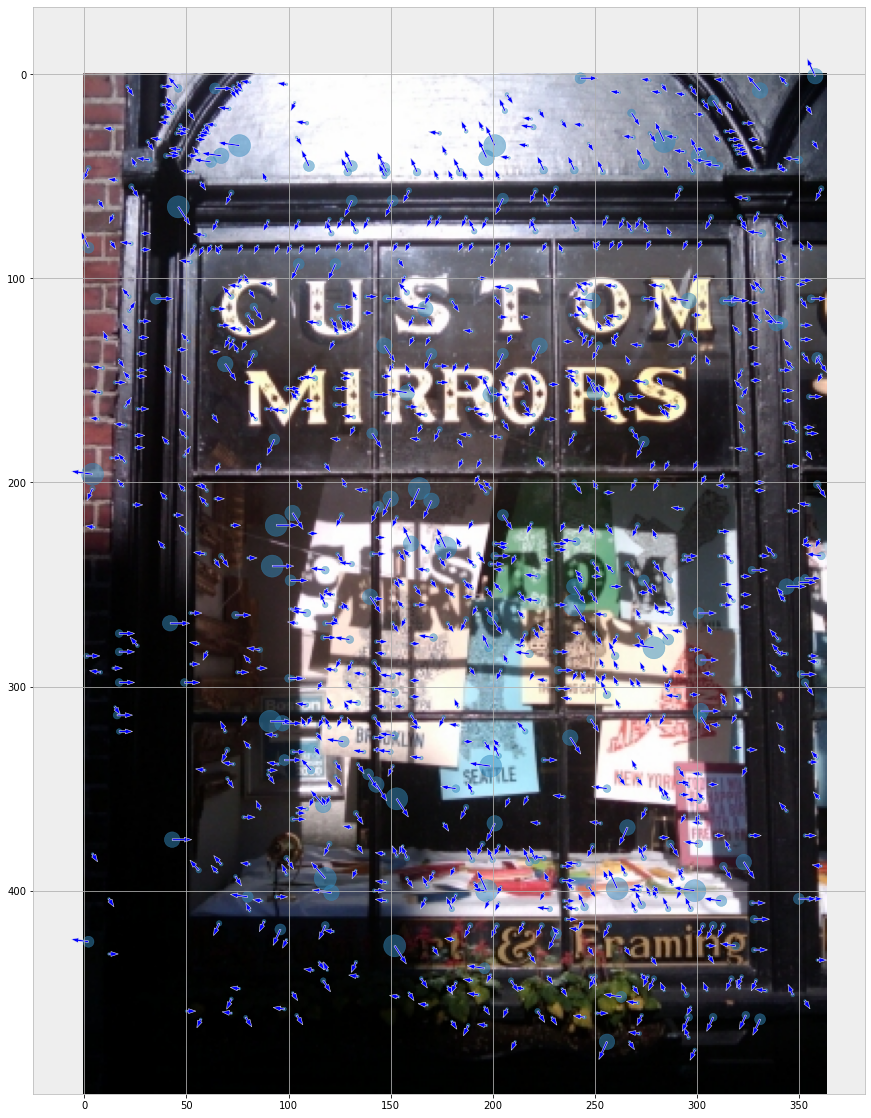
\includegraphics[width=\linewidth]{CustomMirrorsLeftStep3}
	\caption{Left image keypoints with orientation}
	\label{custommirrorsleftstep3}
\end{figure}
\begin{figure}[htb]
	\centering
	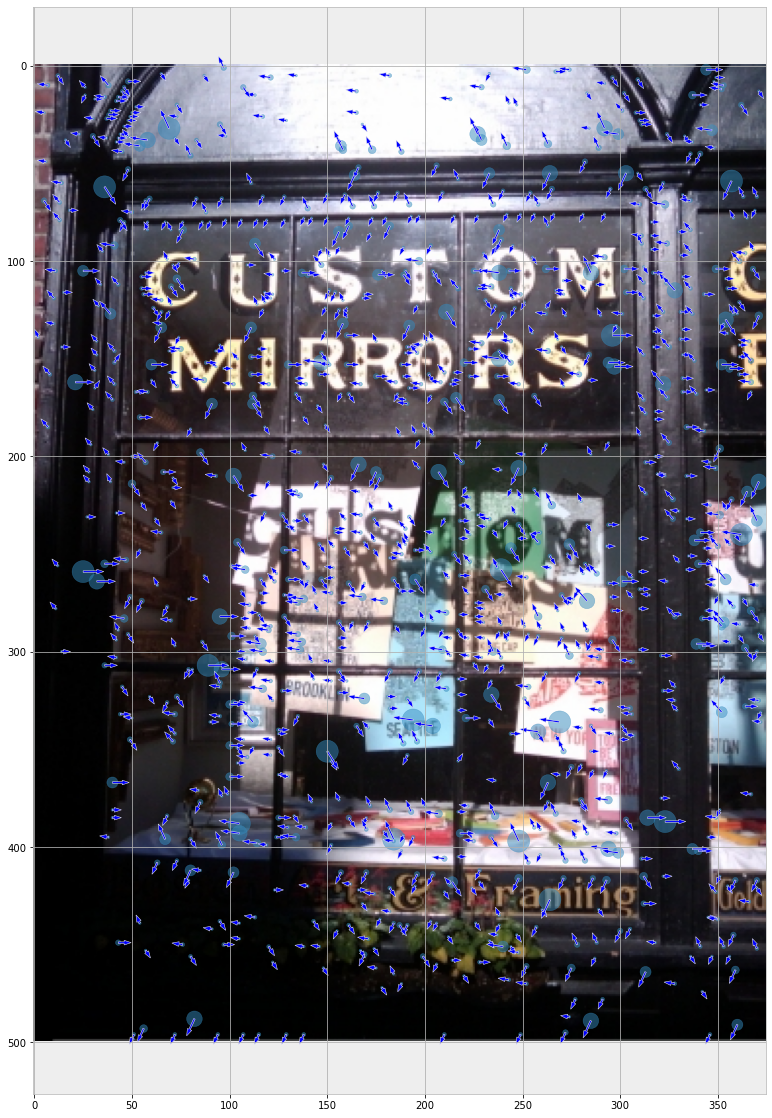
\includegraphics[width=\linewidth]{CustomMirrorsRightStep3}
	\caption{Right image keypoints with orientation}
	\label{custommirrorsrightstep3}
\end{figure}

\begin{figure}[htb]
	\centering
	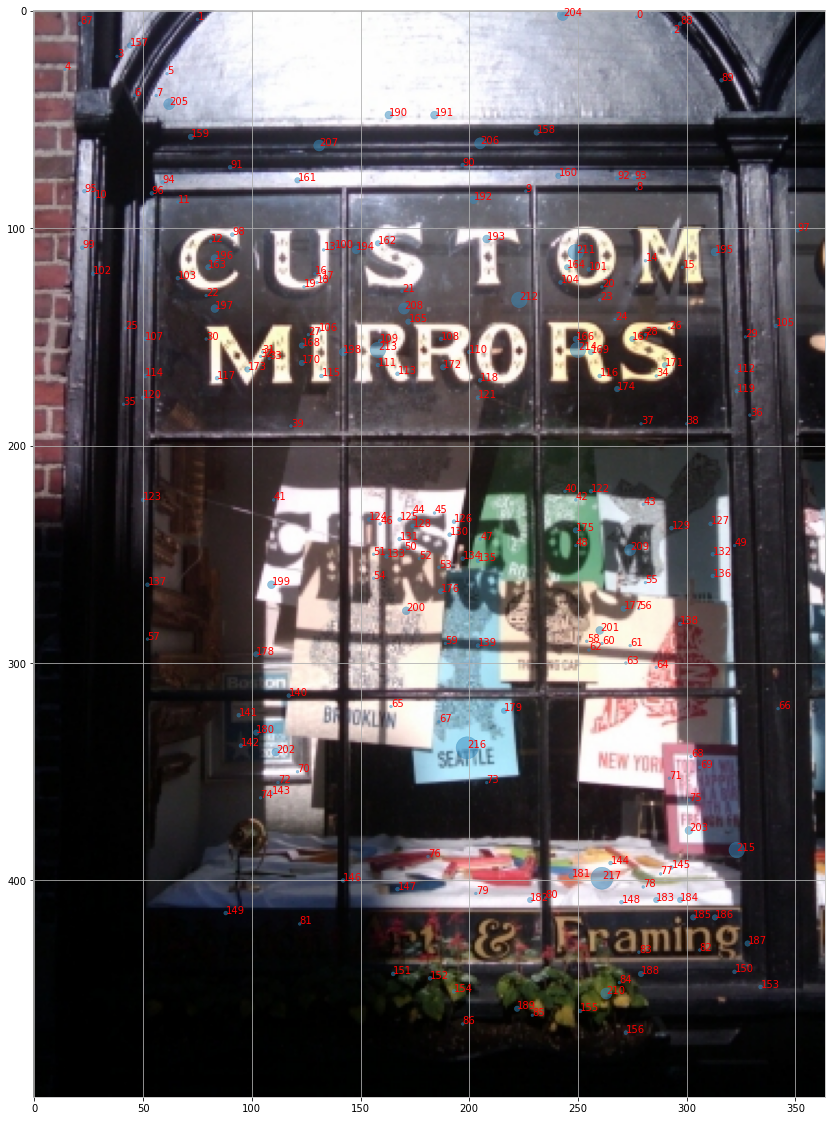
\includegraphics[width=\linewidth]{CustomMirrorsLeftStep4}
	\caption{Left image matched keypoints}
	\label{custommirrorsleftstep4}
\end{figure}
\begin{figure}[htb]
	\centering
	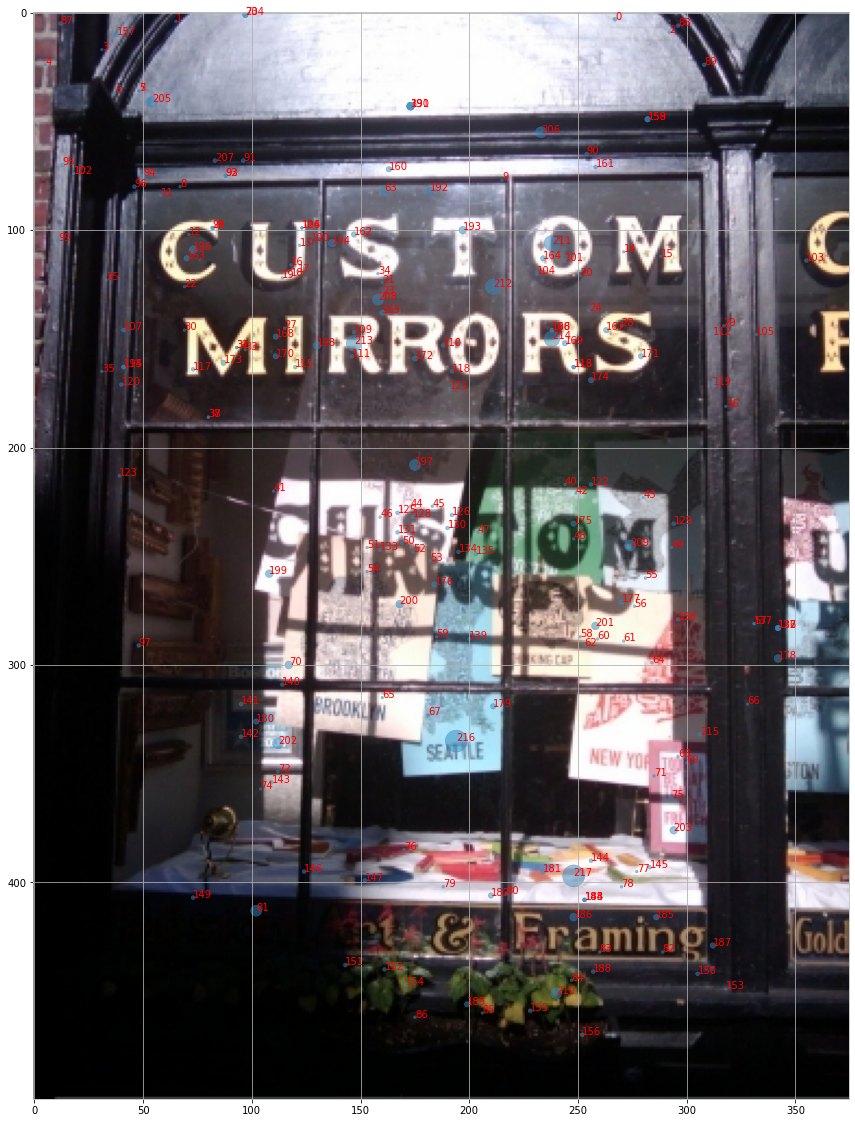
\includegraphics[width=\linewidth]{CustomMirrorsRightStep4}
	\caption{Right image matched keypoints}
	\label{custommirrorsrightstep4}
\end{figure}


\end{document}
